\section{Introduction}
My methodological approach in this project can be divided into three: 
\begin{itemize}
    \item modeling beliefs on players' abilities in a Bayesian manner
    \item modeling FPL's team selection process as a Belief-State Markov Decision Process (BSMDP)
    \item solving the MDP using Bayesian Q-learning
\end{itemize}
This methodology is similar to the one described in the paper - "Competing with Humans at Fantasy Football: Team Formation in Large Partially-Observable Domains" \cite{matthews2012} but with a few alterations. Instead of giving the agent unlimited transfers during the 8th and 23rd gameweeks i.e. playing a Wildcard chip, my agent only got one free transfer per gameweek as per the standard FPL rules. Further, the agent does not utilize any other special chips e.g. free hit, bench boost, assistant manager, and triple captain as described in \ref{ch:special_features}.

I also used team-specific formations while sampling starting lineups for simulated fixtures in the 2022/23 and 2023/24 seasons to provide accurate team composition for my scoring model as depicted in table \ref{tab:fomation_table} 

\section{Modeling players' abilities}
Modeling a player's ability in a manner that captured the uncertainity of their performance in games was important in this project. As such, I took a Bayesian apprach to model this belief by maintaining a distribution over possible performance levels. Furthermore, a Bayesian model allowed me to incorporate domain knowledge through priors using performance data from previous seasons. This was crucial in giving good players a higher baseline even when they experience a slump in their performance. The players' abilities I sought to model are the probabilities of a player: 
\begin{itemize}
    \item scoring a goal
    \item assisting a goal
    \item starting a game
    \item getting subbed during a game
    \item remaining unused during a game
\end{itemize}

\begin{figure}[h]
    \centering
    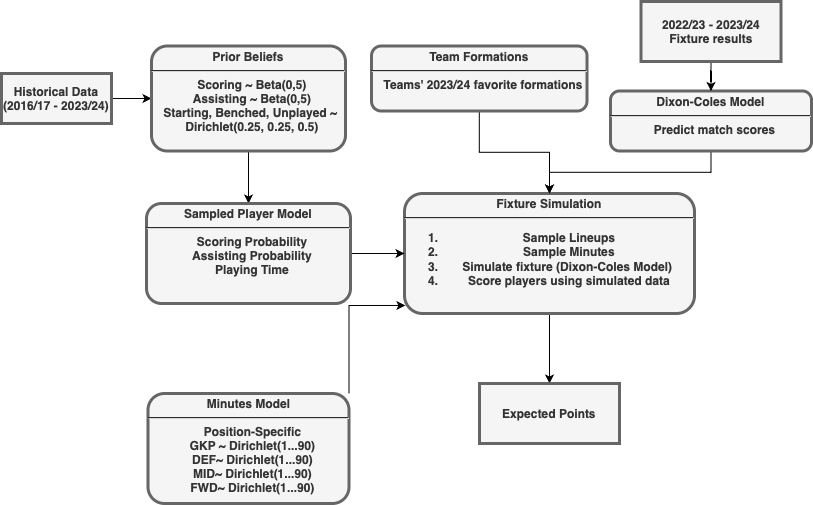
\includegraphics[width=1.2\textwidth]{figs/Bayesian_player_model_Match_simulation.png}
    \vskip 0.2in
    \caption{Bayesian Player Model and Match Simulation}
    \label{fig:bayesian_model_and_simulation}
\end{figure}

Defining the following terms is essential in describing my methodology. For the $i$-th gameweek, we define:
\begin{itemize}
    \item $M_i$ as the set of matches in gameweek $i$.
    \item $P_i$ as the set of players available for selection in gameweek $i$.
    \item $A_i$ as the set of actions available in gameweek $i$, where $a \in A_i$ is a subset of $P_i$ and observes all team selection constraints.
    \item $p_i \in P_i$ is associated with its FPL-designated position $pos(p_i)$ and price $price(p_i)$.
    \item $\tau_p \in \tau$ is a system of distributions representing the player's ability i.e. performance/influence on the matchplay.
    \item $O_i$ is the set of match observations in gameweek $i$.
    \item $o \in O_i$ includes both the result of the matches and the performance of the players in the selected team e.g. goals, assists, clean sheets, yellow cards, red cards, bonus points. The probability of each $o \in O_i$ is somehow dependent on the players' characteristics ($\tau$) i.e. a team with strong attackers is more likely to score goals, therefore, $P(o)$ is dependent on $\tau$.
    \item $R(o, a_{prev}, a_{curr})$ is the reward function, which returns the points scored by the selected team $a_{curr}$, given the match observations $o$. The previous team $a_{prev}$ is also provided to penalize the agent for any poor player transfers.
\end{itemize}

I used three distributions to model players' abilities:
\begin{itemize}
    \item $\rho_p$ - a three-state categorical distribution representing the player's probability of starting a match, being substituted, or not playing at all i.e. (start, sub, unused).
    \item $\omega_p$ - a Bernoulli/Binomial distribution over a single trial, representing the probability of a player scoring a goal given he was playing at the time
    \item $\psi_p$ - a Bernoulli distribution representing the probability of a player providing an assist given he was playing at the time
\end{itemize}
Using a Bayesian approach allowed me to leverage the respective distributions' conjugates to update the players' priors (belief) using data from previous seasons. I defined uniform priors for all players as described in \cite{matthews2012} as follows: $$\omega_p \sim Beta(1, 1), \psi_p \sim Beta(1, 1),  \rho_p \sim Dirichlet(\frac{1}{4}, \frac{1}{4}, \frac{1}{4})$$

I further defined four multinomial distributions $S_{pos}$, one for each position - to describe the how long players who play the same position are likely to play, given they start a match. These distributions were defined using a Dirichlet distribution, modeling the probability a player from the respective position $pos$ leaving the match at minute $x$, where $0 \le x \le 90$. 

Samples of a player's ability, $\tau_p$, and minutes played in a game $S_{pos(p)}$, given they were in the starting lineup, were drawn from these conjugate distributions

I simulated a gameweek by simulating each fixture in the gameweek as follows (The procedure focuses on the home team for conciseness but is also applicable to the away team):
\begin{itemize}
    \item Define $P_H$ and $P_A$ as the set of players available the home and away teams respectively. I used formation frequency data from the English Premier League to determine individual team compositions \cite{clarke2024}. As such, I assigned each team a default formation as shown in table \ref{tab:fomation_table}.
    \begin{table}[h!]
        \centering
        \begin{tabular}{|c|c|}
            \hline
            Team & Formation \\ \hline
            AVL, BHA, BOU, CHE, FUL, MCI, MUN, TOT, WHU & 4-2-3-1    \\ \hline
            ARS, CRY, LIV, NEW & 4-3-3  \\ \hline
            LUT, WOL & 3-4-2-1 \\ \hline
            BRE, SHU & 3-5-1 \\ \hline
            EVE & 4-4-1-1 \\ \hline
            BUR (classic) & 4-4-2 \\ \hline
            NFO & 4-2-3-1 \\ \hline
        \end{tabular}
        \caption{Favored formations for the 2023/24 Premier League Season}
        \label{tab:fomation_table}
    \end{table}
    \begin{itemize}
        \item I, however, had to make some modifications when constituting these teams using the aforementioned formations. In the case where a team does not have enough forwards to fill the required number as per their assigned formation (as was the case with Totttenham (TOT) and Newcastle (NEW)), I used midfielders instead. Further, since Premier League data does not distinguish between attacking and defensive midfielders, I simplified formations with such distinctions e.g. 3-4-2-1 and 4-2-3-1 by grouping both as general midfielders. In this case, my model assigns six midfielders to a 3-(4-2)-1 formation and five to 4-(2-3)-1.
    \end{itemize}
    \item Sample $\tau_p$ for each player $p \in P_H$  from the belief model $Pr(\tau_p | b_i)$
    \item Randomly select eleven players from $P_H$ in proportion to their probability of starting the match i.e. $Pr(\rho_p = start)$ These players constitute the starting lineup $L_H$
    \item The minute each player $p$ leaves the pitch is sampled from the $S_{pos}$ distribution for the player's $pos(p)$
    \item Each player in $P_H$ and not in $L_H$ is assigned to the set of substitutes $U_H$
    \item For every minute that a player in $L_H$ is set to get substituted:
    \begin{itemize}
        \item We randomly select a player from $U_H$ to replace the outgoing player in proportion to the probability of the player being substituted i.e. $Pr(\rho_p = sub)$
        \item The replacement is added to $L_H$ (removed from $U_H$). We further assume that the player being substituted is not substituted again in the same match.
    \end{itemize}
    \item We use the Dixon-Coles model \cite{dixon1997} predict the outcome of the fixture. The model extends the basic Poisson model for soccer prediction by assuming that goals scored by teams follow a Poisson distribution. It also accounts for team-specific attacking and defensive threats, and home advantage while adding a crucial correction for the dependency between team's scores, especially for low-scoring results (0-0, 1-0, 0-1, 1-1). I was fortunate to find a clean implementation of the Dixon-Coles model on David Sheehan's article on "Predicting Football Results with Statistical Modelling: Dixon-Coles and Time-Weighting" \cite{sheehan2018}
    \item If a goal is scored, it is allocated to player $p$ with the following weighted probability. First, we convert the probability of scoring or assisting during a full match into a per-minute rate parameter:
    \begin{align}
    \text{scoring\_rate\_per\_minute} &= \frac{-\ln(1 - \text{score\_prob})}{\text{MATCH\_MINUTES}} \\
    \text{assisting\_rate\_per\_minute} &= \frac{-\ln(1 - \text{assist\_prob})}{\text{MATCH\_MINUTES}}
    \end{align}
    where MATCH\_MINUTES = 90, is the standard length of a soccer game, without accounting for extra time.

    If events (goals/assists) occur according to a Poisson process with constant rate $\lambda$ Then the probability of at least one event occurring in time $t$ is:
    \begin{align}
        P(\text{at least one event in time $t$}) = 1 - e^{-\lambda t}
    \end{align}
    \item Solving for $\lambda$:
    \begin{align}
        P &= 1 - e^{-\lambda t} \\
        1 - P &= e^{-\lambda t} \\
        \ln(1 - P) &= -\lambda t \\
        \lambda &= \frac{-\ln(1 - P)}{t}
    \end{align}
    Once we have the per-minute rates, we recalculate the probability of scoring or assisting based on the actual minutes played:
    \begin{align}
    \text{weighted\_score\_prob} &= 1 - e^{-\text{scoring\_rate\_per\_minute} \times \text{minutes\_played}} \\
    \text{weighted\_assist\_prob} &= 1 - e^{-\text{assisting\_rate\_per\_minute} \times \text{minutes\_played}}
    \end{align}
    This approach accounts for the fact that a player who plays fewer minutes has less opportunity to score or assist. I assume that every goal has anattributed assist and that no one player will score or assist twice in the same game.
    
    \item Other point scoring guidelines i.e. scoring minutes played and clean sheets proceed at described in \ref{ch:scoring_guide}
\end{itemize}
These point estimates were used in combination with the BSMDP reward function $R$ to approximate the immediate reward from performing an action

\section{Modeling the FPL team selection problem}
Similar to the prior problem of modeling players' abilities, selecting an FPL team faces the fundamental problem of making decisions under uncertainity. One doesn't know whether a player will start a game, get injured, or even how long they will play. This is why I opted for a Belief-State Markov Decision Process (BSMDP) as opposed to the standard MDP. The former assumes perfect knowledge of states.

FPL is inherently sequential - decisions in gameweek 1 affect options in gameweek 2 and beyond due to budget constraints, free transfer limitations, and team value changes based on player price fluctuations. As such, the BSMDP naturally captures the sequential nature of FPL team selection.

The Belief State Markov Decision Process is defined by the tuple $(\mathcal{S}, \mathcal{A}, \mathcal{T}, \mathcal{R}, \mathcal{O}, \gamma)$, where:
\begin{itemize}
    \item $\mathcal{S}$ is the state space
    \item $\mathcal{A}$ is the action space
    \item $\mathcal{T}: \mathcal{S} \times \mathcal{A} \times \mathcal{S} \rightarrow [0, 1]$ is the transition function
    \item $\mathcal{R}: \mathcal{S} \times \mathcal{A} \rightarrow \mathbb{R}$ is the reward function
    \item $\mathcal{O}$ is the observation space
    \item $\gamma \in [0, 1)$ is the discount factor
\end{itemize}

In a belief state MDP, the agent maintains a belief distribution over possible states rather than knowing the exact state. We will now formalize each component in the context of the FPL environment.

\subsection{State Space}

The state space $\mathcal{S}$ in the FPL environment is multi-dimensional and consists of:

\[\mathcal{S} = \{(\mathbf{B}, \mathbf{P}, \mathbf{L}, \mathbf{T}, \mathbf{GW}, \mathbf{Z})\}\]

Where:
\begin{itemize}
    \item $\mathbf{B} \in \mathbb{R}^+$ represents the remaining budget (with initial value $B_0 = 100.0$)
    \item $\mathbf{P}$ represents the selected squad of 15 players
    \item $\mathbf{L} \in \mathbf{P}_{15}$ represents the current starting lineup of 11 players 
    \item $\mathbf{T}$ represents the number of free transfers available
    \item $\mathbf{GW} \in \{1, 2, ..., 38\}$ represents the current gameweek
    \item $\mathbf{Z}$ represents the sampled gameweek performances for $p \in A$
\end{itemize}

Each player $p \in \mathcal{P}$ has attributes including:
\begin{itemize}
    \item Position $pos(p) \in \{\text{GK}, \text{DEF}, \text{MID}, \text{FWD}\}$
    \item Captain $cap(p)$ if the player is chosen as the team captain for current gameweek
    \item Likewise for vice captaincy $vice\_cap(p)$. A player can only have one title for a gameweek.
    \item Team $team(p) \in \{1, 2, ..., 20\}$ the team that the player plays for
    \item Price $price(p) \in \mathbb{R}^+$
    \item Expected points $E[points(p, gw)] \in \mathbb{R}^+$ for each gameweek $gw$
\end{itemize}

\subsection{Action Space} \label{action_space}
The action space in our MDP formulatio encompasses all possible valid FPL teams.
However, in the implementation, the action space is simplified to selecting among a subset of three promising actions as suggested in \cite{matthews2012}. I then periodically replaced the weakest member of the simplified action set with a promising member of the unexplored action space.

\begin{align}
\mathcal{A}_{simplified} = \{0, 1, 2\}
\end{align}
where each index corresponds to a dynamically maintained action subset.

The team selection process is solved using linear programming with the PuLP Python Library. The action space is exponential in size since we need to select 15 players from a pool of several hundred, subject to multiple constraints as described in \ref{ch:team_selection_constraints}

Formally, we define binary decision variables $x_i$ for each player $i$, where:
\begin{equation}
    x_i =
    \begin{cases}
        1 & \text{if player $i$ is selected} \\
        0 & \text{otherwise}
    \end{cases}
\end{equation}

Similarly, we define binary variables for the starting lineup:
\begin{equation}
    \text{starter}_i =
    \begin{cases}
        1 & \text{if player $i$ is in the starting 11} \\
        0 & \text{otherwise}
    \end{cases}
\end{equation}
\break
\textbf{Squad composition constraints}
\begin{align}
    \sum_{i \in \mathcal{P}} x_i &= 15 \quad \text{(exactly 15 players)} \\
    \sum_{i \in \mathcal{P}_{\text{GK}}} x_i &= 2 \quad \text{(exactly 2 goalkeepers)} \\
    \sum_{i \in \mathcal{P}_{\text{DEF}}} x_i &= 5 \quad \text{(exactly 5 defenders)} \\
    \sum_{i \in \mathcal{P}{_\text{MID}}} x_i &= 5 \quad \text{(exactly 5 midfielders)} \\
    \sum_{i \in \mathcal{P}_{\text{FWD}}} x_i &= 3 \quad \text{(exactly 3 forwards)}
\end{align}

\textbf{Budget constraint}
\begin{equation}
    \sum_{i \in \mathcal{P}} \text{price}_i \cdot x_i \leq \text{budget}
\end{equation}

\textbf{Team Diversity Constraint}

For each team $t$ in the Premier League:
\begin{equation}
\sum_{i \in \mathcal{P}_t} x_i \leq 3 \quad \text{(maximum 3 players from any team)}
\end{equation}

\textbf{Starting Lineup Constraints}
\begin{align}
    \text{starter}_i &\leq x_i \quad \forall i \in \mathcal{P} \quad \text{(starters must be in squad)} \\
    \sum{i \in \mathcal{P}} \text{starter}i &= 11 \quad \text{(exactly 11 starters)} \\
    \sum{i \in \mathcal{P}_{\text{GK}}} \text{starter}_i &= 1 \quad \text{(exactly 1 starting goalkeeper)} \\
    \sum{i \in \mathcal{P}_{\text{DEF}}} \text{starter}_i &\geq 3 \quad \text{(at least 3 starting defenders)} \\
    \sum{i \in \mathcal{P}_{\text{MID}}} \text{starter}_i &\geq 3 \quad \text{(at least 3 starting midfielders)} \\
    \sum{i \in \mathcal{P}_{\text{FWD}}} \text{starter}_i &\geq 1 \quad \text{(at least 1 starting forward)}
\end{align}

\textbf{Transfer Constraints}
When updating an existing team, we define additional variables for transfers:
\begin{align}
    \text{transfers\_out} &= \sum_{i \in \text{current\_team}} (1 - x_i) \\
    \text{transfers\_in} &= \text{transfers\_out} = 1 (\text{Limit to one transfer})\\
    \text{extra\_transfers} &\geq \text{transfers\_in} - \text{free\_transfers}
\end{align}

\subsection{Transition Dynamics}

The transition function $\mathcal{T}$ for the FPL environment can be decomposed as follows:

\begin{align}
    \mathcal{T}((\mathbf{B}, \mathbf{P}, \mathbf{L}, \mathbf{T}, \mathbf{GW}, \mathbf{Z}), a) = (\mathbf{B}', \mathbf{P}', \mathbf{L}', \mathbf{T}', \mathbf{GW}', \mathbf{Z}')
\end{align}
The transition is deterministic given the action $a$ and the player performance predictions $\mathbf{Z}$.

\subsection{Reward Function}

The reward function $\mathcal{R}$ is defined as the points earned in a gameweek minus any transfer penalties. The captain's points are counted twice as per FPL special features \ref{ch:special_features}

\begin{align}
\mathcal{R}((\mathbf{B}, \mathbf{P}, \mathbf{L}, \mathbf{T}, \mathbf{GW}, \mathbf{Z}), a) &= \sum_{p \in \mathbf{L - cap(p)}} points(p, GW) \nonumber \\
&\quad + 2*points(cap, GW) - transfer\_cost
\end{align}

Where:
\begin{itemize}
    \item $transfer\_cost = 4 \times \max(0, num\_transfers - free\_transfers)$
\end{itemize}


\section{Solving the FPL team selection Problem}
Bayesian Q-learning is particularly well-suited for solving the FPL BSMDP since it directly incorporates uncertainty about the value function itself. Rather than maintaining a point estimate of Q-values as in standard Q-learning, it maintains a probability distribution over possible Q-values. This helps deal with uncertainities about the true value of performing an action i.e. choosing a team $a \in \mathcal{A}$. Further, it makes better use of the relatively few data points (38 gameweeks), by incorporating prior knowledge from previous gameweeks.

For each potential action $a$, the agent maintains a belief distribution over the Q-value as follows:

\begin{align}
    Q(s, a) \sim \mathcal{NG}(\mu_{a}, \lambda_{a}, \alpha_{a}, \beta_{a})
\end{align}

Where $\mathcal{NG}$ is a Normal-Gamma distribution with:
\begin{itemize}
    \item $\mu_{a}$: mean estimate of the Q-value
    \item $\lambda_{a}$: precision parameter
    \item $\alpha_{a}$: shape parameter
    \item $\beta_{a}$: rate parameter
\end{itemize}

\subsection{Bayesian Q-Value Update}

After taking action $a$ and observing reward $r$, the belief distribution is updated according to the normal-gamma update rules:

\begin{align}
\lambda_{a}' &= \lambda_{a} + 1\\
\alpha_{a}' &= \alpha_{a} + 0.5\\
\mu_{a}' &= \frac{\lambda_{a} \mu_{a} + r}{\lambda_{a}'}\\
\beta_{a}' &= \beta_{a} + \frac{0.5 \lambda_{a} (r - \mu_{a})^2}{\lambda_{a}'}
\end{align}

\subsection{Value of Perfect Information (VPI)}
The environment uses the Value of Perfect Information (VPI) to balance exploration and exploitation as suggested in \cite{matthews2012}. For the best known action $a_1$, we only learn anything from performing it if $q*_{
a1}$ is now lower than the currently estimated Q-value of $a_2$, $\hat{q_{a2}}$, the second-best action. Likewise, for all $a \neq a_1$, we only learn anything from performing $a$ if $q_a$ is now greater than $\hat{q_{a1}}$. The extent by which $q_a$ is greater than $\hat{q_{a1}}$ represents the gain in knowledge
(and vice-versa for $a_1$). For each action $a$, the VPI is calculated as:

\begin{align}
VPI(a) = \begin{cases}
\sigma_a \cdot t_{\nu}(z) \cdot (1 - CDF_{\nu}(z)) + \sigma_a \cdot PDF_{\nu}(z) & \text{if } a = a^*\\
\sigma_a \cdot z \cdot CDF_{\nu}(z) + \sigma_a \cdot PDF_{\nu}(z) & \text{if } a \neq a^*
\end{cases}
\end{align}

Where:
\begin{itemize}
    \item $a^*$ is the action with the highest estimated mean Q-value
    \item $\nu = 2\alpha_a$ is the degrees of freedom for the t-distribution
    \item $\sigma_a = \sqrt{\frac{\beta_a(1+1/\lambda_a)}{\alpha_a}}$ is the standard deviation
    \item $z = \frac{Q(a') - \mu_a}{\sigma_a}$ where $Q(a')$ is the Q-value of the best alternative action if $a = a^*$, or the Q-value of the best action if $a \neq a^*$
    \item $CDF_{\nu}$ and $PDF_{\nu}$ are the cumulative distribution function and probability density function of the t-distribution with $\nu$ degrees of freedom
\end{itemize}

\subsection{Action Selection and Exploration}

The action selection mechanism combines exploitation (choosing the action with the highest estimated Q-value) with directed exploration using VPI:

\begin{align}
a_{selected} = \arg\max_a \{\mu_a + VPI(a)\}
\end{align}

Additionally, the environment dynamically updates the action subset by replacing actions with low utility (defined as $\mu_a + VPI(a) < \mu_{a^*}$) with newly generated promising actions as described in \ref{action_space}. \cite{matthews2012}

\subsection{Algorithm}
The initial team is selected greedily based on expected points:
The team is selected to maximize the sum of sampled points while respecting the constraints on team composition, budget, and players per team.
The overall algorithm for the FPL Belief State MDP is presented in \ref{alg:bayesianQLearning}:

\begin{algorithm}
\caption{Bayesian Q-Learning Algorithm}
\begin{algorithmic}[1]
\State Initialize team $\mathbf{T}$ with players having highest expected points for $GW = 1$
\State Initialize budget $B = B_0$
\State Initialize gameweek $GW = 1$
\State Initialize action subset with promising transfers
\State Initialize Bayesian Q-values $\mathcal{NG}(\mu_a, \lambda_a, \alpha_a, \beta_a)$ for each action
\While{$GW \leq 38$}
    \State Select action $a = \arg\max_a \{\mu_a + VPI(a)\}$ 
    \State Execute transfer if specified by $a$
    \State Observe reward (gameweek points - transfer cost)
    \State Update Bayesian Q-values using observed reward and VPI for all actions
    \State Update players' priors based on performances
    \State Replace low-utility actions with new promising actions if necessary
    \State $GW = GW + 1$
\EndWhile
\end{algorithmic}
\label{alg:bayesianQLearning}
\end{algorithm}

\section{Data Collection Methods}
Implementing this project would not have been possible without clean, publicly-available data sources. 

The most important data source was the gameweek-by-gameweek data in the \\ \href{https://github.com/MUN3N3Z/FPL_AI/tree/main/data}{\underline{data folder}} of my code repository that was cloned from the FPL Historical Dataset. The dataset is available in this \href{https://github.com/vaastav/Fantasy-Premier-League/tree/master}{\underline{Github repository}} \cite{anand2016fantasypremierleague}.

While I later discovered that I could have retrieved season fixtures by manipulating the data from the forementioned repository, I ended up scraping fixture data from the official Fantasy Premier League API using a \href{https://github.com/MUN3N3Z/FPL_AI/tree/main/scripts/save_season_fixtures.py}{\underline{Python script}}

I also scraped fixture results i.e. home team, away team, home team goals, and away team goals from \href{www.football-data.co.uk}{\underline{football-data website}}

\section{Technology Stack}
\subsection{Hardware Infrastructure}

\begin{itemize}
    \item Computational resources: Apple M2 Chip, 8 GB Ram, 256 GB Memory
    \item Computing environment: Local workstation
\end{itemize}

\subsection{Software framework}
\begin{itemize}
    \item Operating System: macOS Sequoia 15.4.1
    \item Programming Languages: Python
    \item Integrated Development Environment (IDE): Visual Studion Code
    \item Version Control: Git, GitHub
\end{itemize}

\subsection{Data Management}
\begin{itemize}
    \item Data Storage: GitHub, Local
    \item Data Format: CSV, Pickled Python objects
    \item Data Processing Tools: Pandas
\end{itemize}

\subsection{Analysis \& Modeling}
\begin{itemize}
    \item Statistical Analysis Tools: Numpy, Pymc
    \item Machine Learning Libraries: Scipy (optimization), Gymnasium, PuLP \\(optimization)
    \item Visualization Tools: Matplotlib
    \item Domain-Specific Libraries: \href{https://fpl.readthedocs.io/en/latest/}{\underbar{FPL API Python Wrapper}} \cite{macLeod2019}
\end{itemize}

\subsection{Reproducibility Framework}
\begin{itemize}
    \item Environment Management: Miniconda virtual environment ``fpl\_env''
    \item Dependency Management: Miniconda 
    \item Random Seed Control: Set RANDOM\_SEED variable in constants.py
\end{itemize}

